\documentclass[conference]{IEEEtran}
\IEEEoverridecommandlockouts
% The preceding line is only needed to identify funding in the first footnote. If that is unneeded, please comment it out.
\usepackage{cite}
\usepackage{amsmath,amssymb,amsfonts}
\usepackage{algorithmic}
\usepackage{graphicx}
\usepackage{textcomp}
\usepackage{xcolor}
\usepackage{balance}

\usepackage[nohyperlinks, printonlyused, nolist]{acronym}

\usepackage[utf8]{inputenc}
\usepackage[T1]{fontenc} % Trennen von Wörtern mit Umlauten
\usepackage{ngerman} % Damit z.B. "Literatur" statt "References" da steht


\def\BibTeX{{\rm B\kern-.05em{\sc i\kern-.025em b}\kern-.08em
    T\kern-.1667em\lower.7ex\hbox{E}\kern-.125emX}}
\begin{document}

\begin{acronym}
    \acro{apt}[APT]{Advanced Persistent Threat}
    \acro{bsi}[BSI]{Bundesamt für Sicherheit in der Informationstechnik}
    \acro{opsec}[OpSec]{Operational Security}
    \acro{fbi}[FBI]{Federal Bureau of Investigation}
    \acro{cisa}[CISA]{Cybersecurity and Infrastruktur Security Agency}
    \acro{odni}[ODNI]{Office of the Director of National Intelligence}
    \acro{nsa}[NSA]{National Security Agency}
    \acro{ttp}[TTP]{Taktik, Technik und Prozedur}
    \acro{hsg}[HSG]{High-Level Szenario Graph}
    \acro{masfad}[MASFAD]{Multi-agent System for Advanced Persistent Threat Detection}
\end{acronym}


\title{Methoden und Techniken von \aclp*{apt} am Beispiel des SolarWinds Compromise
}

\author{\IEEEauthorblockN{Laurenz Stinner}
    \IEEEauthorblockA{\textit{Fakultät für Informatik} \\
        \textit{Technische Hochschule Rosenheim}\\
        Rosenheim, Germany \\
        laurenz.p.stinner@stud.th-rosenheim.de}
}

\maketitle

\begin{abstract}
    \acp{apt} sind ein große Gefahr für jedes Netzwerk. Ihre besonderen Eigenschafen ermöglichen es \acp{apt} in nahezu jedes Netzwerk einzudringen.
    In der Arbeit wird zunächst erklärt, wie sich \acp{apt} von anderen Formen der Cyberkriminalität unterscheiden und wie diese im allgemeinen Vorgehen.
    Anschließend wird gezeigt wie die \ac{apt}29 im Fall des SolarWinds Compromise vorgegangen ist.
    Zum Schluss werden Verteidigungsmaßnahmen wie Threat Hunting und das MASFAD Framework vorgestellt.
\end{abstract}

\begin{IEEEkeywords}
    \ac{apt}, SolarWinds Compromise, Cybersecurity, APT, Cloudsecurity, Threat Hunting, Killchain, MASFAD
\end{IEEEkeywords}

\section{Einführung}
\label{sec:introduction}

Laut Statista belaufen sich die geschätzten jährlichen weltweiten Kosten von Cyberkriminalität auf 8,15 Billionen US-Dollar und steigen bis 2028 um 69,94\% auf 13,82 Billionen US-Dollar an \cite{Statista2023}.
In Deutschland entstehen durch Cyberattacken Schäden in Höhe von 148 Milliarden Euro, was 72\% des gesamten Schadens etspricht, der durch Industriespionage, Sabotage und Datendiebstahl verursacht wird.
Besonders im Zuge des russischen Angriffskrieg auf die Ukraine hat das \ac{bsi} viele Phänomene bezüglich Cyberkriminalität in Deutschland festgestellt \cite[S.~25]{BSI2023}.
Das \ac{bsi} gibt an, das im Durchschnitt täglich 250.000 neue Varianten von Schadprogrammen bekannt werden \cite[S.~13]{BSI2023}.
Dies macht deutlich, wie wichtig es ist, zu verstehen wie \acp{apt} agieren, um sich bestmöglich auf Angriffe dieser Art vorzubereiten.

\subsection{Organisierte Kriminalität, Hacker und \aclp*{apt}}
\label{sec:introduction:apt}

Bei der Cyberkriminalität wird zwischen verschiedenen Formen unterschieden, siehe Abb.~\ref{fig.destinction}.
\begin{figure}[htbp]
    \centerline{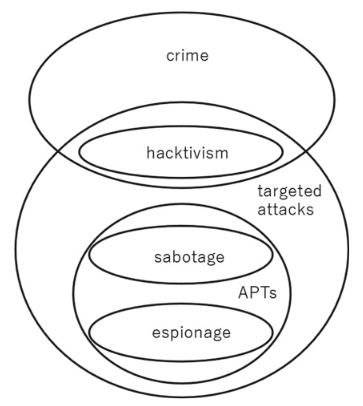
\includegraphics[scale=0.8]{figures/Destinction between targeted attacks, activity by APTs, and cyber-espionage.png}}
    \caption{Unterscheidung zwischen gezielten Angriffen, Aktivitätes von \acp{apt} und Cyberspionage \protect\cite[S.~6]{Steffens2020}}
    \label{fig.destinction}
\end{figure}
Das National Institute of Standards and Technology beschreibt \acp{apt} wiefolgt:
Als \acp{apt} werden Gruppierungen oder Personen bezeichnet, die über ein hohes Maß an Fachwissen und erhebliche Ressourcen verfügen, die es Ermöglichen mehrere Angriffsvektoren zu nutzen.
Zusätzlich verfolgen \acp{apt} ihre Ziele wiederholt über einen längeren Zeitraum, passen sich den Bemühungen der Verteitiger an und sind entschlossen die Ziele zu erreichen.
Zu diesen Zielen gehören u.~a. das Exfiltrieren von Informationen, kritische Aspekte einer Organisation zu stören und sich im System des Ziels zu verbreiten und festzusetzen \cite[S.~B-1]{NIST2011}.

\subsection{SolarWinds Compromise \& APT29}
\label{sec:introduction:solarwinds}

Der SolarWinds Compromise war eine Supply-Chain-Attacke der Gruppe \ac{apt}29 und wurde im Dezember 2020 entdeckt \cite{MITRESolarwindsCompromise}.
Das betroffene Softwareprodukt war die Orion Platform des Unternehmens SolarWinds.
Die Platform ermöglicht das Überwachen, Analysieren und Verwalten von Resourcen in Cloudumgebungen \cite{OrionPlatform}.
Dieser Umfang an Fuktionen hat die Platform zu einem Ziel gemacht, da durch eine mögliche Schwachstelle sehr viele Systeme betroffen sind, was letztendlich eingetreten ist.
Der Angriff war so weitreichend, dass das \ac{fbi}, \ac{cisa}, \ac{odni} und die \ac{nsa} eine gemeinsame Erklärung \cite{JointStatement} zu dem Angriff herausgegeben haben.
Lt. diesem Bericht waren ca. 18.000 öffentliche und private Kunden der Software SolarWinds Orion betroffen.
Eine erheblich kleinere Zahl der Kunden wurde durch nachfolgende Aktivitäten kompromittiert.
Die Erklärung enthält bereits die Indizien, dass die verantwortliche \ac{apt} russischen Ursprungs ist.

Die USA und das Vereinigte Königreich verantworten gemeinsam den russischen Auslandsgeheimdienst für den Angriff \cite{USUKSVR}.
Die Gruppe erhält in späteren öffentlichen Erklärungen u.~A. die Beinamen APT29 und Cozy Bear \cite{CybersecurityAdvisoryAPT29}.

\ac{apt}29 operiert seit mindestens 2008 und haben es primär auf Regierungsnetzwerke in Europa und NATO-Mitgliedsstaaten, Forschungsinstitute und Denkfabriken abgesehen \cite{MITREAPT29}.
MITRE ordnet der \ac{apt}29 neben dem SolarWinds Compromise auch die Operation Ghost zu \cite{MITREAPT29}.

\section{Vorgehensweise von \aclp{apt}}

Die Techniken der \acp{apt} werden immer komplexer und vielfältiger und bestehen aus vielschichtigen und zeitaufwändigen Prozessen \cite[S.~7f]{Steffens2020}.
Um sie besser zu verstehen, werden die verschiedenen Teile eines Anriffs in eine \textit{killchain} sortiert \cite[S.~8]{Steffens2020}, siehe Abb.~\ref{fig.killchain}.
\begin{figure}[htbp]
    \centerline{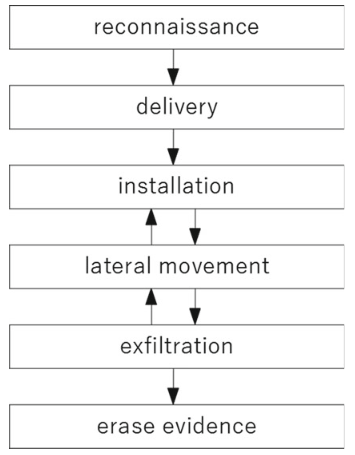
\includegraphics[scale=0.8]{figures/killchain.png}}
    \caption{Killchain: Idealisiertes Modell der Stufen eines \ac{apt}-Angriffs \cite[S.~8]{Steffens2020}}
    \label{fig.killchain}
\end{figure}
Es gibt weitere Killchain-Modelle, u.~a. von Lockheed Martin \cite{LockheedMartin}, welche einfachheitshalber nicht weiter in betracht genommen werden.
MITRE unterscheidet sogar noch detailierter zwischen den verwendeten Taktiken \cite{MITREEnterpriseTactics}.

Im Folgenden werden die Schritte der \textit{Killchain} aus Abb.~\ref{fig.killchain} erklärt und Taktiken gelistet die durch \acp{apt} genutzt werden, um das Ziel des Schrittes zu erreichen.

\subsection{Aufkärung}

Das Ziel des ersten Schritts ist es nicht nur Information über das Ziel zu finden, sondern auch das Ziel festzulegen.
Wie und warum Ziele ausgewählt werden lässt sich schwer bis nicht feststellen.
Meist wird angenommen, dass \acp{apt} einen Auftrag durch Kunden bekommen, beispielsweise durch Geheimdienste, und danach ihre Ziele suchen.
Nachdem das Ziel feststeht beginnt die weitere Aufklärung.
Vgl. zu diesem Abschnitt Steffens \cite[S.~10ff]{Steffens2020}.

In der Regel werden öffentlich zugängliche Informationen über ein Ziel gesammelt, um dessen Arbeitsweise besser zu verstehen und potenzielle Angriffsvektoren zu identifizieren \cite{Cole2013}.

MITRE \cite{MITREReconnaissance} listet zehn Techniken auf, mit deren Hilfe Informationen über das Ziel gefunden werden können:
\begin{itemize}
    \item \textbf{Active Scanning} - Direkte Interaktion mit der Infrastruktur des Ziels (IP-Adressblöcke finden, Schwachstellenscanns, Wortlistsuche)
    \item \textbf{Gather Victim Host Informatiomn} - Harware- und Softwareinformation über das Zielsystem finden (Betriebssystem, Konfigurationen, Firmware, usw.)
    \item \textbf{Gather Victim Identity Information} - Informationen über Mitarbeiter (Daten von Personen, E-Mail Adressen, Zugangsdaten)
    \item \textbf{Gather Victim Network Information} - Grundlegende Informationen über das Netzwerk (IP-Adressen, DNS- \& Domain-Informationen, Netzwerktopologie, usw.)
    \item \textbf{Gather Victim Org Information} - Informationen über das Unternehmen sammeln, die für weiter Schritte genutzt werden können (Geschäftsbeziehungen, Personalstruktur und -hierarchie, usw.)
    \item \textbf{Phishing for Information} - Erlangen von vertraulichen Informationen mithilfe von u.~a. Social-Engineering Taktiken (Telefonate, E-Mails, usw.)
    \item \textbf{Search Closed Sources} - Informationen über das Ziel kaufen (Dark-Web Schwarzmärkte, usw.)
    \item \textbf{Search Open Technical Databases} - Technische Informationen über das Ziel in frei verfügbaren Online-Datenbanken finden (WHOIS, DNS, CDNs, usw.)
    \item \textbf{Search Open Websites/Domains} - Informationen über Suchmaschienen, Social-Media oder Coderepositorien finden.
    \item \textbf{Search Victim-Owned Websites} - Durchsuchen von Webseiten nach Informationen, die dem Ziel gehören (E-Mail Adressen, Mitarbeitername, usw.)
\end{itemize}
Viele der Techniken werden kombiniert, um am Ende das eigentliche Ziel zu erreichen.
Beispielsweise werden auf der Webseite des Ziels wichtigen Mitarbeitern gesucht, weitere Informationen über Social-Media gewonnen, um anschließend vertrauliche Informationen über das Ziel mittels Social-Engineering Taktiken zu gewinnen.

\subsection{Auslieferung}
\label{sec:proceeding:delivery}

Die Auslieferung ist sehr verbunden mit der Aufklärung.
Häufig wird für eine gewählte Auslieferungsstrategie entsprechende Aufklärung durchgeführt.
Wird beispielsweise der Angriffsvektor E-Mail ausgewählt, müssen vorab über diverse Aufklärungstaktiken Informationen gefunden werden, um zu gewährleisten, dass beispielsweise der Inhalt der Mail geöffnet wird.
Vgl. zu diesem Abschnitt Steffens \cite[S.~10ff]{Steffens2020}.

MITRE \cite{MITREInitialAccess} bezeichnet diesen Schritt als initialen Zugriff und unterscheidet zwischen zehn Techniken:
\begin{itemize}
    \item \textbf{Content Injection} - Nutzen von bereits kompromittierten Datenübertragungskanälen.
    \item \textbf{Drive-by Compromise} - Ziel wird aktiv zu bösartigen Nutzdaten auf einer kompromittierten Webseite gelockt, z.~B. Abgreifen von Anwendungszugriffstoken.
    \item \textbf{Exploit Public-Facing Application} - Ausnutzen einer Schwachstelle eines Systems.
    \item \textbf{External Remote Services} - Nutzen von unzureichend abgesicherten Remote-Diensten, wie VPNs.
    \item \textbf{Harware Additions} - Einbringen neuer Hardware in ein System oder Netzwerk, z.~B. Wechseldatenträger.
    \item \textbf{Phishing} - Versenden von Phishing-Nachrichten, um einen Zugang zum System des Ziels zu erhalten.
    \item \textbf{Replication Through Removable Media} - Eindringen in abgetrennte Netzwerke, z.~B. mittels Wechselmedien in Kombination mit Autorun-Funktionen
    \item \textbf{Supply Chain Compromise} - Einschleusen von bösartigem Code durch Auslieferungsmechanismen von Anwendungen.
    \item \textbf{Trusted Relationship} - Ausnutzen von vertrauenswürdigen Dritten, um Zugang zu einem Netzwerk zu erhalten.
    \item \textbf{Valid Accounts} - Nutzen von Anmeldeinformationen bestehender Konten (VPNs, Outlook, Remote-Desktop, ...)
\end{itemize}
Viele Angriffe von \acp{apt} werden im nachhinein durch IT-Sicherheitsunternehmen beschrieben, jedoch ist es meist unmöglich herauszufinden, wie die Angreifer in das Netzwerk gelangt sind \cite[S.~14]{Steffens2020}.
Wie in Abschnit~\ref{sec:introduction:apt} beschrieben, verfügen \acp{apt} über erhebliche Ressource und können desshalb über Wochen oder Monate hinweg den Angriff ausführen.
In dieser Zeit können Angreifer ihre Spuren verwischen, bzw. viele Unternehmen halten Log-Dateien nicht entsprechend lange vor, um diese Auswerten zu können \cite[S.~15]{Steffens2020}.

\subsection{Installation}

Ziel dieses Schritts ist es die Kontrolle über ein System im Netzwerk des Ziels zu bekommen.
Der Schritt Auslieferung, aus Abschnitt~\ref{sec:proceeding:delivery}, und dieser Schritt sind in der Regel die größte Herausforderung und entscheidend für den Erfolg eines Angriffs.
Im Zuge diese Schritts wird eine Verbindung zwischen dem kompromittierten System und einem \textit{Control Server} mittels sog. \textit{Backdoors} hergestellt, um den Zugriff zu tarnen.
Vgl. zu diesem Abschnitt Steffens \cite[S.~15]{Steffens2020}.

MITRE \cite{MITREEnterpriseTactics} unterscheidet in diesem Punkt zwischen Taktiken für die Ausführung von schadhaftem Code, \textit{Execution}, und Taktiken, um den Zugriff auf längere Zeit zu sichern \cite{MITREEnterpriseTactics}.
Zu den Taktiken für die Ausführung von schadhaftem Code listet MITRE \cite{MITREExecution} folgende auf:
\begin{itemize}
    \item \textbf{Cloud Administration Command} - Missbrauchen von Cloud-Verwaltungsdiensten, wie AWS Systems Manager und Azure Runcommand.
    \item \textbf{Command and Scripting Interpreter} - Befehls- und Skriptinterpreter, wie Unix-Shell und PowerShell, werden zum ausführen von schadhafem Code verwendet.
    \item \textbf{Container Administration Command} - Über Containerverwaltungsdienste kann schadhafter Code innerhalb eines Containers ausgeführt werden.
    \item \textbf{Deploy Container} - Einsetzen von schadhaften Containern, um beispielsweise Prozesse auszuführen die Malware ausführen oder herunterladen.
    \item \textbf{Exploitation for Client Execution} - Ausnutzern von Software-Schwachstellen in Client-Anwendungen, um Code auszuführen.
    \item \textbf{Inter-Process Communication} - Manipulieren von prozessübergreifender Kommunikation, um Befehle oder Code auszuführen.
    \item \textbf{Native API} - Verwenden von nativen Betriebssystemschnittstellen.
    \item \textbf{Scheduled Task/Job} - Ermöglicht bösartigen Code erstmalig oder wiederholt auszuführen, indem Fuktionen zur Aufgabenplanung missbraucht werden.
    \item \textbf{Serverless Execution} - Missbrauchen von Serverless Computing, Integrations- und Automatisierungsdiensten, um Code in Cloudumgebungen auszuführen.
    \item \textbf{Shared Modules} - Schadhafter Code kann über gemeinsame Module (z.~B. DLLs) ausgeführt werden.
    \item \textbf{Software Deployment Tools} - Bei Zugang zu installierten drittanbieter Softwares für Systemadministration, -monitoring und Softwarebereitstellung kann beliebe Malware in großen Teilen des Netzwerks installiert werden. Dadurch wird auch die Verbreitung im Netzwerk erzielt.
    \item \textbf{System Services} - Verwenden von Systemdiensten oder Daemons zur Ausführung von Code. Kann bereits zum erreichen von Persistenz verwendet werden.
    \item \textbf{User Execution} - Bösartiger Code wird hierbei durch einen Benutzer ausgeführt, der durch Social Engineering dazu gebracht wurde.
    \item \textbf{Windows Management Instrumentation} - Ausnutzen der Windows Management Insturmentation, um Befehle auszuführen.
\end{itemize}

Die größte Teil der genannten Taktiken ermöglichen es, schadhaften Code einmalig auszuführen, jedoch werden diese Prozesse nach neustart eines Systems beendet.
Um den Zugang über Neustarts hinweg zu sichern, werden Taktiken zu persistierung eingesetz \cite{MITREPersistence}.
Dazu gehören nach MITRE \cite{MITREPersistence} folgende Taktiken:
\begin{itemize}
    \item \textbf{Account Manipulation} - Aktionen um den Zugriff auf ein Konto aufrechtzuerhalten. z.~B. durch Ändern von Anmeldedaten.
    \item \textbf{BITS Jobs} - Windows Brackground Intelligent Transfer Services (BITS) können genutzt werden um Malware als Hintergrundaufgabe dauerhaft auszuführen.
    \item \textbf{Boot or Logon Autostart Execution} - Systemeinstellungen konfigurieren, damit ein Programm bei Systemstart oder Anmeldung automatisch ausgeführt wird.
    \item \textbf{Boot or Logon Initialization Scripts} - Verwendung von Skripten die automatisch beim Booten oder bei der Anmeldung auseführt werden.
    \item \textbf{Browser Extensions} - Missbrauchen von Browser-Erweiterungen, um sich dauerhaften Zugang zu verschaffen.
    \item \textbf{Compromise Client Software Binary} - Schadhaften Code in Client-Software-Binärdateien einschleusen.
    \item \textbf{Create Account} - Eigenes Konto für den Systemzugang erstellen.
    \item \textbf{Create or Modify System Process} - Erstellen oder Ändern von Prozessen auf Systemebene (z.~B. Windows-Dienste). Diese werden beim Start des Betriebssystems hochgefahren.
    \item \textbf{Event Triggered Execution} - Mit Hilfe von Systemmechanismen können bei bestimmten Ereignissen Prozesse ausgeführt werden. Besonders in Cloud-Umgebungen, werden Cloud-Ereignisse überwacht und bei entsprechende Ereignissen Funktionen oder Dienste ausgeführt.
    \item \textbf{External Remote Services} - Über Remote-Dienste kann der Zugriff auf ein Netzwerk persistiert werden (z.~B. VPNs).
    \item \textbf{Hijack Execution Flow} - Missbrauch der Art und Weise, wie Betriebssystem Programme ausführen (Ausführungsfluss). Durch umgeleitete Ausführungen kann schadhafter Code immer wieder geladen werden.
    \item \textbf{Implant Internal Image} - Einsetzen von schadhaftem Code in Cloud- oder Container-Images.
    \item \textbf{Modify Authentication Process} - Modifizieren von Authentifizierungsmechanismen- und -prozessen, um auf Benutzeranmeldeinformationen zuzugreifen.
    \item \textbf{Office Application Startup} - Verwendung von Office-Vorlagenmakros oder Add-Ins, um schadhaften Code in Office-basierten Anwendungen zu persistieren.
    \item \textbf{Power Settings} - Beeinträchtigen der Systemfunktionen in den Ruhezustand zu gehen, neu zu starten oder herunterzufahren, um zu verhindern, dass schadhafter Code gestoppt wird.
    \item \textbf{Pre-OS Boot} - Nutzen von Pre-OS-Boot-Mechanismen, um während des Bootvorgangs schadhafte Firmware und verschiedene bösartige Startdienste vor dem Betriebssystem zu laden.
    \item \textbf{Scheduled Task/Job} - Erstellen oder Modifizieren von geplanten Aufgaben, um schadhaften Code wiederholt auszuführen.
    \item \textbf{Server Software Component} - Ausnutzen von legitimen, erweiterbaren Entwicklungsfunktionen von Servern, die ermöglichen Software oder Skripte zu schreiben und zu installieren.
    \item \textbf{Traffic Signaling} - Verbergen von offenen Ports oder anderen bösartigen Funktionen. Ein magischer Wert oder eine Sequenz muss verwendet werden, um eine Reaktion auf dem System auszulösen, z.~B. das Öffnen eines Ports oder die Ausführung einer bösartigen Aufgabe.
    \item \textbf{Valid Accounts} - Durch erbeutete Anmeldeinformationen bestehender Konten, können diese Wiederholt missbraucht werden, um den Zugriff aufrechtzuerhalten.
\end{itemize}

Neben MITRE beschreibt auch Steffens die Kombination mehrerer Techniken, um das Ziel zu erreichen \cite[S.~16]{Steffens2020}.
Trotz der erheblichen Ressourcen die einer \ac{apt} zur Verfügung stehen, werden durch die wenigsten \textit{zero-day exploits} verwendet, denn meist sind genügend alte Sicherheitslücken vorhanden \cite[S.~15]{Statista2023}
Bereits 2019 wurden 70\% der Angriffe über MS Office Produkte ausgeführt \cite{Statista2019}, was Steffens auf die Makro- und Skript-Funktionalität der Office-Produkte zurückführt \cite[S.~15]{Steffens2020}
Trotz standardmäßige Blockierung von Skripten und Makros in Office-Produkten \cite{nicholasswhite2023}, schaffen es Angreifer die Benutzer dazu zu verleiten diese auszuführen.

\subsection{Verbreitung}
\label{sec:proceeding:lateralmovement}

Besonders dieser Schritt ist charakteristisch für \acp{apt}, denn andere Angreifer beschränken sich normalerweise auf ein System, um beispielsweise Zugangsdaten von Onlinebanking zu stehlen.
Zunächst müssen auf dem kompromittierten System erweiterte Rechte ergattert werden.
Hierzu werden Techniken zur \textit{privilege escalation} eingesetzt.
Vgl. dazu Steffens \cite[S.~16f]{Steffens2020}.

MITRE \cite{MITREPrivilegeEscalation} listet hierzu die folgenden Techniken:
\begin{itemize}
    \item \textbf{Abuse Elevation Control Mechanism} - Umgehen von Mechanismen zur Kontrolle der Berechtigungserweiterung, um sich höhere Berechtigungen zu verschaffen.
    \item \textbf{Access Token Manipulation} - Verändern eines Zugriffstokens, sodass z.B.~ ein Prozess so aussieht, als gehöre er zu einem Benutzer mit erweiterten Berechtigungen.
    \item \textbf{Account Manipulation} - Manipulieren von Kontent, um den Zugang zu erweitern.
    \item \textbf{Boot or Logon Autostart Execution} - Systemeinstellungen so konfigurieren, dass Programme bei Systemstart oder Anmeldung automatisch mit erweiterten Berechtigungen gestartet werden.
    \item \textbf{Boot or Logon Initialization Scripts} - Verwenden von Skripten, die beim Booten oder der Anmeldung eines Benutzers mit erweiterten Berechtigungen ausgeführt werden und somit in dessen Sicherheitskontext laufen.
    \item \textbf{Create or Modify System Process} - Erstellen von Prozessen auf Systemebene die u.~U. mit Administrationsberechtigungen ausgeführt werden \cite{MITRECreateOrModifySystemProcess}.
    \item \textbf{Domain Policy Modification} - Verändern von beispielsweise Domänen-Gruppenrichtlinien, um die Berechtigungen innerhalb der Domäne zu erweitern.
    \item \textbf{Escape to Host} - Ausbrechen aus einem Container, um auf das zugrunde liegende Hostsystem zuzugreifen.
    \item \textbf{Event Triggered Execution} - Mit Hilfe von Systemmechanismen Code bei bestimmten Ereignissen ausführen, der mit erweiterten Berechtigungen startet.
    \item \textbf{Exploitation for Privilege Escalation} - Ausnutzen von Software-Schwachstellen, um die Berechtigungen zu erweitern.
    \item \textbf{Hijack Execution Flow} - Missbrauchen der Art und Weise wie Betriebssysteme Programme ausführt. Dabei werden in den Ausführungsfluss schadhafter Code oder schadhafte Nutzdaten eingeschleust und diese u.~U. mit erweiterten Berechtigungen verarbeitet.
    \item \textbf{Process Injection} - Hierbei wird Code in einen Prozess eingeschleust. Läuft der Prozess mit erweiterten Berechtigungen, wird auch der eingeschleuste Code mit diesen Berechtigungen ausgeführt.
    \item \textbf{Scheduled Task/Job} - Ausnutzen der Aufgabenplanung eines Systems. Geplante Aufgaben können u.~U. mit erweiterten Berechtigungen ausgeführt werden.
    \item \textbf{Valid Accounts} - Verschaffen von Anmeldeinformation bestehender Konten, die bereits erweiterte Berechtigungen haben.
\end{itemize}

Einige dieser Taktiken werden auch in anderen Schritten verwendet, wesshalb die klare Abtrennung zwischen den Schritten nicht ganz so leicht möglich ist.
Nachdem Angreifer administrative Berechtigungen erlangt haben, wird das System z.~B. auf Anmeldeinformation zu anderen System durchsucht, um mit Hilfe dieser auf andere Systeme im Netzwerk zu gelangen \cite[S.~17]{Steffens2020}.
MITRE \cite{MITRELateralMovement} kennt einige weitere Taktiken, um sich im Netzwerk zu verbreiten:
\begin{itemize}
    \item \textbf{Exploitation of Remote Services} - Ausnutzen eines Remote-Dienstes innerhalb eines Netzwerkes, um sich unerlaubten Zugang zu weiteren internen Systemen zu verschaffen. Dabei werden Software-Schwachstellen in Programmen und Betriebssystemen ausgenutzt.
    \item \textbf{Internal Spearphishing} - Angreifer können sich mittels internem Spearphishing Zugang zu zusätzlichen Information verschaffen. Es handelt sich dabei um ein mehrstufiges Verfahren, bei dem z.~B. ein E-Mail-Konto eines Benutzers in Besitz genommen wird.
    \item \textbf{Lateral Tool Transfer} - Übertragen von Tools oder anderen Dateien zwischen Systemen in einer kompromittierten Umgebung.
    \item \textbf{Remove Service Session Hijacking} - Kontrolle über bereits bestehende Sitzungen in Remote-Diensten übernehmen.
    \item \textbf{Remote Services} - Verwenden von gültigen Kontent, um sich bei einem Dienst anzumelden, der Remote-Verbindungen akzteptiert, z.~B. SSH.
    \item \textbf{Replication Through Removable Media} - Wechselmedien können verwendet werden, um sich auch in getretten Netzwerken zu verbreiten. Dabei wird Malware auf das Wechselmedium gespielt und mittels Autorun-Funktion auf dem getrennten System ausgeführt.
    \item \textbf{Software Deployment Tools} - Zugang zu Softwarebereitstellungssystemen von Drittanbietern zu verschaffen, um diese zur Verbreitung zu nutzen.
    \item \textbf{Taint Shared Content} - Schadprogramme auf gemeinsam genutzten Speicherorten (Netlaufwerke, Code-Repositorien) in vertrauenswürdigen Dateien ablegen. Sobald ein Nutzer den freigegebenen Inhalt öffnet, kann so der Schadcode verbreitet werden.
    \item \textbf{Use Alternate Authentication Material} - Verwenden von alternativem Authentifizierungsmaterial (Kennwort-Hashes, Kerberos-Tickets, Token, usw.), um sich weiter im System zu verbreiten.
\end{itemize}

In Abb.~\ref{fig.killchain} ist zu sehen, dass \textit{installation}, \textit{lateral movement} und \textit{exfiltration} als Kreislauf dargestellt werden.
Dies erklärt Steffens damit, dass für Systeme die durch die Verbreitung zugreifbar werden der Zyklus erneut beginnt und die Schritte durchlaufen werden \cite[S.~18]{Steffens2020}.

\subsection{Exfiltration}

Die Exfiltration von Dokumenten und Daten ist das eigentliche Zeil von \acp{apt}, die anderen Schritte sind nur ein Mittel zum Zweck.
Im Groben geht es darum, die Dokumente und Daten an einen Server zu übermitteln der unter voller Kontrolle der \ac{apt} steht.
Dafür greifen \acp{apt} auf Wortlisten zurück, um nach interessanten und relevaten Daten zu filtern.
Dabei werden Dokumentnamen, Ordnernamen oder auch Dateiendungen berücksichtigt, die einen Hinweis auf wichtige Daten liefern.
Einerseits wird dieses Vorgehen gewählt, damit der Aufwand des Durchsuchens der Dateien realisierbar bleibt, andererseits birgt das Exfiltrieren großer Datenmengen die Gefahr schneller entdeckt zu werden, da ungewöhnlich großer Netzwerkverkehr erzeugt wird.
Vgl. dazu Steffens \cite[S.~18]{Steffens2020}.

MITRE \cite{MITREExfiltration} listet dafür folgende Taktiken auf:
\begin{itemize}
    \item \textbf{Automated Exfiltration} - Automatisches exfiltrieren von z.~B. sensiblen Dokumenten. Dafür wird diese Technik meist mit anderen Exfiltrationstechniken kombiniert \cite{MITREAutomatedExfiltration}.
    \item \textbf{Data Transfer Size Limit} - Exfiltrieren von Daten in kleineren Paketen, um z.~B. zu vermeiden, dass Schwellenwerte für die Datenübertragung im Netzwerk nicht überschritten werden.
    \item \textbf{Exfiltration Over Alternative Protocol} - Daten über andere Protokolle, als das der bestehenden Verbindung, exfiltrieren.
    \item \textbf{Exfiltration Over C2 Channel} - Daten über das Protokol der bestehenden Verbindung exfiltrieren.
    \item \textbf{Exfiltration Over Other Network Medium} - Nutzen von anderen Netwerkmedien, wie WiFi-Verbindungen, mobile Datenverbindungen oder Bluetooth, um Daten zu exfiltrieren.
    \item \textbf{Exfiltration Over Physical Medium} - Stehlen von Daten mittels physischer Medien, z.~B. USB-Laufwerke oder Mobiltelefone.
    \item \textbf{Exfiltration Over Web Services} - Verwenden von Webdiensten zur Exfiltration, z.~B. über Fileshare-Dienste.
    \item \textbf{Scheduled Transfer} - Planen von Datenexfiltrationen, damit nur zu bestimmten Tageszeiten oder in bestimmten Zeitabständen. Diese Taktik wird u.~U. genutzt, um den Datenverkehr mit normalen Aktivitäten zu vermischen. Andere Taktiken werden meist mit dieser verbunden \cite{MITREScheduledTransfer}.
    \item \textbf{Transfer Data to Cloud Account} - Übertragen von Daten, einschließlich Backups von Cloud-Umgebungen, auf ein anderes Cloud-Konto, um Exfiltrationserkennung zu umgehen.
\end{itemize}

In der Regel werden Dateien die exfiltriert werden sollen zuvor in passwortgeschützte und komprimierte Archive RAR gepackt, um das Opfer daran zu hindern, herauszufinden welche Dateien gestohlen wurden \cite[S.~19]{Steffens2020}.

\subsection{Beweise löschen}
Die sog. \ac{opsec} korreliert stark mit der Raffinesse von \acp{apt}.
Besonders Gruppen die der NSA und CIA zugeordnet werden, sind stark im Thema \ac{opsec}.
Dabei geht es darum genutzte Tools zu löschen, Logs richtig zu löschen und sonstige Spuren zu entfernen oder zu verwischen, um zu verhindern entdeckt zu werden.
Viele \acp{apt} führen diesen Schritt nicht sorfältig durch.
Dadurch lassen sich viele Spuren finden, aber nicht alle.
Viele System löschen selbst die Spuren von Anreifern, z.~B. durch Logrotation.
Zusätzlich wird dieser Schritt gemieden, da gute System das Löschen von Logs überwachen und Alarm schlagen.
Vgl. dazu Steffens \cite[S.~19f]{Steffens2020}.

\section{Vorgehensweise im SolarWinds Compromise}

Der Angriff auf SolarWinds wurde als Supply-Chain-Attacke eingestuft, was bedeutet, dass das Ziel des Angriffs nicht SolarWinds selbst, sondern die Kunden von SolarWinds waren.
Das US-amerikanische Cybersicherheitsunternehmen FireEye entdeckte als erstes den Angriff \cite{9579611}.

Da keine festen Beweise gefunden wurden, wie \ac{apt}29 auf die internen System von SolarWinds gelangt sind, um in deren Software eine Backdoor einzubauen, wird im Folgenden nur die Kompromittierung der Kunden von SolarWinds analysiert.
Dabei wird der Angriff auf eine nicht näher benannte us-amerikanische Denkfabrik genauer betrachtet, der durch das Unternehmen Volexity beobachtet wurde.

\subsection{Zeitlicher Ablauf}
Der Begin der Attacke wird auf den 06.08.2019 datiert, dort wurde die erste bekannte Infrastruktur für die Attacke angelegt.
Die erste Modifikation der SolarWinds Software geht auf den 26.10.2019 zurück, wobei die erste ausnutzbare Schwachstelle in den Softwareupdates ab März 2020 enthalten war, die als SUNBURST-Malware bezeichnet wird.
Am 13.12.2020 wurde der SolarWinds Report von Fireeye veröffentlicht und somit der Angriff öffentlich bekannt.
Ein Tag später wurde von SolarWinds ein Sicherheitshinweis zur Attacke herausgegeben.
Am 15.12.2020 wurde die SUNBURST C2 (Command and Control) Domaine durch Microsoft beschlagnahmt \cite{Unit2020}.
Im durch Veloxity beobachteten Angriff wurde im Juli 2020 die Malware in SolarWinds Orion ausgenutzt \cite{Cash2020}.

\subsection{Aufklärung}
Die Aufklärungsphase ist im SolarWinds Compromise etwas schwammig.
Die Malware SUNBURST, die durch ein Update der SolarWinds Orion Platform mit installiert wurde, dient u.~A. dazu, Aufklärung im Netzwerk der Opfer zu betreiben \cite{Intelligence2020}.
Jedoch wurde die Malware zuerst ausgeliefert und installiert, wesshalb hier die Reihenfolge der Killchain nicht exakt wiedergegeben wird.
Wie in Abb.~\ref{fig.killchain} vermerkt ist, ist die Killchain auch nur ein idealisiertes Modell, und der SolarWinds Compromise unterstützt diese Aussage durch das verdrehen der Schritte.

\subsection{Auslieferung und Installation}
Die Malware SUNBURST wurde durch ein Softwareupdate durch authorisierte Systemadministratoren heruntergeladen und installiert \cite{FIREEYE2020}.

SUNBURST wurde in die SolarWinds.Orion.Core.BusinessLayer.dll eingeschleust.
Dort wurde die Malware in einer Methode aktiviert die in regelmäßigen Abständen aufgerufen wurde.
Das stellte sicher, dass die Persistenz der Malware gewährleistet ist und neustart eines Systems immer wieder ausgeführt wurde.
Neben einigen Bedingungen, prüft die Malware vor ihrem Start, ob Prozesse laufen, die einer Sicherheitssoftware zugeordnet werden können, um sich vor diesen zu verstecken.
Sobald die Malware gestartet ist, baut sie eine Verbindung zu einem C2 (Command and Control) Server auf, um grundlegende Informationen über das System zu übermitteln.
Über den C2 Server können Befehle an die Malware übermittelt werden und ermöglichen eine vollen Zugriff auf das System \cite{Intelligence2020}.

\subsection{Erneute Aufklärung}
Im durch Veloxity beobachteten Angriff wurde nach dem Eindringen in das Netzwerk erneut Aufklärungsarbeit betrieben.
Es wurden mittels Powershell Konfigurationseinstellung im Exchange der Organisation ausgelesen.
Darunter befanden sich Informationen über Exchange-Nutzer und deren aktuellen Rollen.
Vgl. zu diesem Abschnitt Cash et al. \cite{Cash2020}.

\subsection{Verbreitung}
Um sich im Netzwerk zu verbreiten erstellten die Angreifer mittels PowerShell neue geplante Aufgaben auf weiteren Systemen \cite{Cash2020}.

\subsection{Exfiltration}
Der Zugriff auf den Exchange Server der Denkfabrik ermöglichte es den Angreifern via PowerShell-Kommands Mailboxen zu extrahieren.
Diese wurden in ein passwort-geschütztes Archiv verpackt, um durch eine HTTP-Anfrage exfiltriert werden zu können.
Um Verteidigungsmechanismen zu umgehen wurde das Archiv als PNG Bilddatei über eine URL zur verfügung gestellt.
Zusätzlich fügten die Angreifer ein eigenes Gerät als zulässige ID für die aktive Synchronisierung für eine Reihe an Postfachern hinzu, um weiterhin Zugriff auf die Postfächer zu erhalten.
Vgl. zu diesem Abschnitt Cash et al. \cite{Cash2020}.

\subsection{Beweise löschen}
Nach der erfolgreichen Exfiltration der E-Mails, wurde die Export-Anfrage aus dem Exchange Server gelöscht.

\section{Verteidigung gegen \aclp{apt}}
\subsection{Threat Hunting}
Unter Theat Hunting versteht man die Kombination von Netwerkverkehr, Logs, Code und anderen mehrquelligen Daten, um den Host, Angriffspfad, den Angreifer und die Angrifssorganisation, die den Angriff gestartet hat, durch die verschiedenen Techniken und Methoden zu lokalisieren \cite{Chen2022}.
Sicherheitsunternehmen haben in den letzten Jahren viele Forschungsberichte zu \ac{apt}-Angriffen veröffentlicht, jedoch meist nach den Angriffen \cite{Chen2022}.
Durch die Entwicklung von Deep-Learning und traditionellen maschinellen Lern-Technologien, hat es fortschritte bezüglich Erkennung und Rückverfolgung von \ac{apt}-Angriffen basierend auf der Analyse von Provenance Graphen gegeben \cite{Chen2022}.
\subsubsection{UNICORN}
UNICORN ist ein Angriffserkennungssystem, welches versucht Angriffe auf mehrere Hosts gleichzeitig zu erkennen \cite{Han2020}.
\begin{figure*}[htbp]
    \centerline{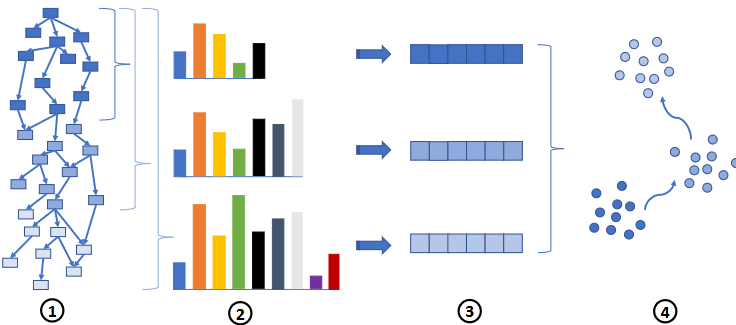
\includegraphics[scale=0.6]{figures/UNICORN.png}}
    \caption{Schematischer Aufbau von UNICORN; Quelle: \cite{Han2020}}
    \label{fig.unicorn}
\end{figure*}
Als Eingabe nutzt UNICORN einen Provenence Graphen mit benannten Kanten, der dauerhaft aktualisiert wird.
Daraus wird ein Histogramm konstruiert, siehe Abb.~\ref{fig.unicorn} Schritt 2, wobei jedes Histogrammelement eine eindeutige Substruktur des Graphen beschreibt.
UNICORN reduziert dabei den Einfluss von Histogrammelementen, die in keinen kausalen Zusammenhang mit den aktuellen Ereignissen im System stehen.
Aufgrund der Datenmenge wendet UNICORN eine ähnlichkeitserhaltende Hashing-Technik an und wandelt so das Histogramm in eine Graphenskizze um, siehe Abb.~\ref{fig.unicorn} Schritt 3.
Daraus erstellt UNICORN ein normales Systemausführungsmodell und identifiziert abnormale Aktivitäten ohne Wissen über Angriffe.
Dafür erfasst das Modell Verhaltensänderungen innerhalb einer einzelnen Ausführung, indem es Systemaktivitäten in verschiedenen Phasen der Ausführung clustert und Veränderungen erkennt.
Das Modell wird dabei nicht dynamisch während der Laufzeit angepasst, desshalb ist es besser geeignet für lang laufende Systeme, die vorher analysiert werden können.
Vgl. zu diesem Abschnitt Han et al. \cite{Han2020}.
\subsubsection{HOLMES}
HOLMES ist ein System, welches versucht aus Ereignisspuren auf effiziente Weise Alarme zu generieren.
\begin{figure*}[htbp]
    \centerline{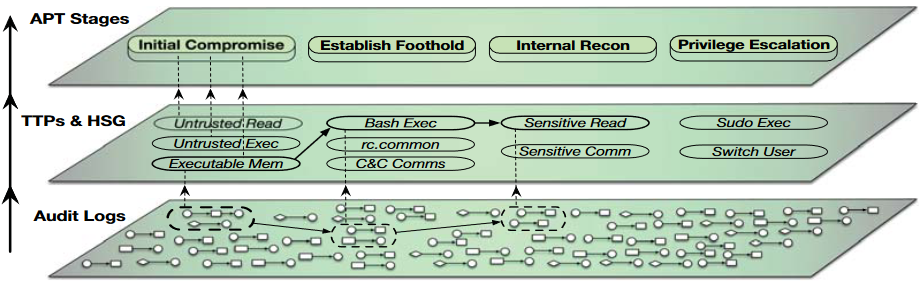
\includegraphics[scale=0.5]{figures/HOLMES.png}}
    \caption{Schematischer Aufbau von HOLMES; Quelle: \cite{Milajerdi2019}}
    \label{fig.holmes}
\end{figure*}
Zuerst sammelt HOLMES Audit-Protokolle von veschiedenen Systemen, die Ereignisse, von beispielsweise Dateiveränderungen, Prozessen und Netzwerkverbindungen, enthalten.
Diese Daten werden in einem Provenance Graphen abgebildet, bei dem die Knoten des Graphen Subjekte (Prozesse) und Objekte (Dateien, Sockets) bilden und die Kanten die Abhängigkeiten mit Ereignisnamen zwischen diesen darstellen.
Zur weiteren Verarbeitung der Daten ist eine Sammlung an Taktiken, Techniken und Prozeduren von \acp{apt} nötig.
Diese Sammlung verbindet \acp{ttp} mit Ereignissen, Vorbedingungen und Schweregrad und Gruppiert diese in die Schritte der Killchain.
Aus dem Graphen der Ereignisse und der Sammlung von \acp{ttp} wird ein \ac{hsg} erstellt.
Bei diesem bilden die Knoten die \acp{ttp} ab, die Kanten den Informationsfluss zwischen den Elementen die zur \ac{ttp} zugeordnet sind.
Dazu wird der Provenance Graph nach den Vorbedingungen der \acp{ttp} analysiert und wenn alle Vorbedingugen einer \ac{ttp} erfüllt sind, wird diesen in den \ac{hsg} hinzugefügt.
Um den  \ac{hsg} zu bewerten, wird aus den \acp{ttp} der höchste Schweregrad einer \ac{ttp} der Aufklärungsphase gewählt.
Vgl. zu diesem Abschnitt Milajerdi et al. \cite{Milajerdi2019}.

\subsection{Visuelle Analytik mit dem MASFAD-Framework}
Das \ac{masfad} bietet die Möglichkeit \acp{apt} mittels Anomalie- und verhaltensbasierter Analyse zu erkennen.
Dabei fokusiert sich das Framework auf das erkennen von zuvor nicht erkannter oder unbekannter Bedrohungen.
\ac{masfad} konzentriert sich stärker auf die von verschiedenen Sensoren im Netzwerk gesammelten Daten, als auf die Topologie des Netzwerks.
Dabei steht der Analyst selbst im Mittelpunkt und dessen Fachwissen wird durch die vorgeschlagene Visualisierung von \ac{masfad} erweitert.
Durch die verschiedenen Visualisierungsformen sollen dem Analysten die Daten verständlich aufbereitet werden und verhelfen korrekte Annahmen über Aktivitäten im Netzwerk zu treffen.
Vgl. zu diesem Abschnitt Nikolov und Mees \cite{Nikolov2023}.

\section{Fazit}
\ac{apt} sind Aufgrund ihres Durchhaltevermögens eine besondere Gefahr für Unternehmen, Regierungen und sonstige Organisationen.
Die in der Arbeit gezeigte Vorgehensweise von \acp{apt} macht deutlich, wie Aufwändig und Schwierig es ist sie zu erkennen, gar zu bekämpfen.
Das zeigt besonders der SolarWinds Compromise der sogar amerikanische Behörden bedroffen hat, die selbst in der Informationssicherheit tätig sind.
Durch diverse Maßnahmen wie Mitarbeiterschulungen und gute Systemadministration können zwar Hürden geschaffen werden, jedoch keine \ac{apt} wirklich davon abgehalten werden, das System zu kompromittieren.
Wird ein Weg blockiert, sucht sich eine finanzkräftige und personenstarke \ac{apt} den nächsten Weg und wiederholt alles, bis das Ziel erreicht ist.

Die vorgestellten Verteidigungstechniken wie HOLMES, UNICORN und das \ac{masfad}-Framework können bei der Sicherung von Systemen unterstützend wirken.
Jedoch sind Ressource, v.~a. Fachpersonal, weiterhin notwendig, um die Erkenntnisse der Verteidigungstechniken anzuwenden.

\balance
\bibliographystyle{IEEEtran}
\bibliography{IEEEexample}
\end{document}
